\section{Experiment 1: Simulated Data from Multivariate Normal Distribution}

In the first simulation experiment, we focused on an ideal setting where data come from a known multivariate normal 
distribution and imputation is required to estimate the mean, variance and covariances of six items with missing values.
We investigated the relative performance of the methods described in Section \ref{secMethods} across a set of conditions 
defined by two experimental factors: the number of columns in the dataset $p$, taking values 50 or 500; 
and the proportion of \emph{per} variable missing cases $pm$, taking values 0.1 or 0.3.
Table \ref{tab:condExp1} summarizes the four crossed conditions.
Data with sample size $n=200$ were independently generated 1,000 times for each set of conditions.
For each replicate, missing values were imposed and then all the missing data treatment methods described above
were used to obtain estimates for the parameters of a substantive analysis model of interest.

\begin{table}
	\centering
	\begin{tabular}{l | r | r | r }
		condition & n & p & pm \\
		\hline
		1 & 200 & 50  & .1 \\
		2 & 200 & 500 & .1 \\
		3 & 200 & 50  & .3 \\
		4 & 200 & 500 & .3 \\
	\end{tabular}
	\caption{\label{tab:condExp1}Summary of conditions for experiment 1.}
\end{table}

\FloatBarrier % stops table:condSum leaving its own section

\subsection{Simulation Study Procedure}

\subsubsection{Data Generation}
	A data matrix $\bm{Z}_{n \times p}$ was generated according to a multivariate normal model centered
	around a mean of 0 with a covariance matrix $\bm{\Sigma}_0$, with diagonal elements (variances) equal to 1.
	The off-diagonal elements of $\bm{\Sigma}_0$ were used to define three blocks of variables: 
	the first five variables were highly correlated among themselves ($\rho = .6$);
	variables 6 to 10 were weakly correlated with variables in block 1 and among themselves ($\rho = .3$), 
	and all the remaining $p-10$ variables were uncorrelated.
	Items were rescaled to have mean of 5.

\subsubsection{Missing Data Imposition} \label{sub_missing}

	Missing values were imposed on six items in $\bm{Z}_{n \times p}$: three variables in the block of
	highly correlated variables ($z_j$ with $j = 1,2,3$), and three in the block of lowly correlated variables ($z_j$ 
	with $j = 6,7,8$).
	Item non-response was imposed by sampling from a Bernoulli distribution with individual probabilities defined by 
%
	\begin{equation} \label{eqn:rm}
		p_{miss} = p(z_{i,t} = miss | \tilde{Z}) = \frac{ exp(\gamma_0 + \tilde{Z}_{i}\bm{\gamma}) }
								{ 1 + exp(\gamma_0 + \tilde{Z}_{i}\bm{\gamma}) }
	\end{equation}
%
	where $z_{i,j}$ is the $i$-th subject's response on the $j$-th variable target of missing data imposition, 
	$\tilde{Z}_{i}$ is a vector of responses for the $i$-th individual to the set of predictors involved in 
	the missing data mechanism, $\gamma_0$ is the intercept parameter, and $\bm{\gamma}$ is the vector of slope 
	parameters.
	$\tilde{Z}$ was specified to include two fully observed variables from the highly correlated set, and two 
	from the lowly correlated set ($z_r$ with $r = 4,5,9,10$).	
	The choice of predictors in $\tilde{Z}$ is important to allow imputations under MAR: 
	the probability of observing a response for a target variable did not depend on the variable itself, 
	to avoid imputation under Missing Not At Random; and, as all features in the data are included in the MI 
	procedures, the predictors in $\tilde{Z}$ are always allowed to be part of the imputation models.
	All slopes in $\bm{\gamma}$ were fixed to 1, while the value of $\gamma_0$ was chosen with an optimization algorithm that 
	minimized the difference between a target proportion of missing values and its actual value.

\subsubsection{Imputation}
	
	Missing values were treated with all the methods described in Section 2.
	For both experiments, convergence of the imputation models was assessed in a preprocessing step.
	Before running the actual simulation studies, 10 datasets were generated according to each experimental set up.
	Missing values in each dataset were imputed by running 5 parallel imputation chains for each Multiple Imputation 
	method.
	Convergence was checked by plotting the mean of the imputed values for each variable in each stream, against the 
	iteration number.
	In each parallel run, all the MI algorithms run for 250 iterations.
	In the simulation experiments, the imputation algorithms were considered to converge after 50 iterations, 
	after which 10 imputed data sets were store and used for the subsequent standard complete-data analysis and 
	pooling.
	The only exception was blasso, which required approximately 2000 iterations for convergence.

	The ridge penalty used in the bridge algorithm is fixed across iterations and its value needs to be
	decided beforehand by the imputer.
	The value used in the simulation was determined by means of cross-validation in a pre-processing phase.
	The grid of possible values for the ridge penalty was $10^{-1}, 10^{-2}, ..., 10^{-8}$.
	For each of 100 data repetitions, bridge imputation was performed with each of the different penalty parameters
	and used to obtain 10 differently imputed datasets.
	For each data replication, the Fraction of Missing Information (FMI) \citep{savaleiRhemtulla:2012} associated with each 
	parameter in the analysis models of interest (see next section for details) was computed and then averaged across 
	repetitions.
	The mean of these average parameter FMIs was used as a composite measure of FMI associated with each ridge penalty
	value.
	Finally, the penalty value with the smallest composite FMI was selected.
		
	Both IURR and DURR could have been specified with a variety of penalty parameters.
	For example, one could use any of the following: ridge penalty \citep{hoerlKennard:1970}, lasso penalty 
	\citep{tibshirani:1996}, elastic net penalty \citep{zouHastie:2005}, adaptive lasso \citep{zou:2006}.
	In this study we specified the regularization as a lasso penalty as it is computationally efficient, and it 
	performed well for imputation in \cite{zhaoLong:2016} and \cite{dengEtAl:2016}.
	A 10-fold cross-validation procedure was used at every iteration of DURR and IURR to choose the penalty parameter.

	For blasso, in order to maintain consistency with previous research, the hyperparameters in equations 
	\eqref{eqn:sigprior}, \eqref{eqn:tauprior}, and \eqref{eqn:rhoprior} were specified as in \cite{zhaoLong:2016}: 
	$(a,b)=(0.1, 0.1)$, $(r,s)=(0.01, 0.01)$, and $(g,h)=(1,1)$.
	In the MI-PCA algorithm, enough components were extracted to explain 50\% of the total variance in the data.
	To impute data with the single imputation random forest approach we used the function \emph{missForest} in the 
	homonymous R package.
	This function implements algorithm 1 proposed by \cite{stekhovenBuhlmann:2011}.
	The stopping criterion for the missForest algorithm was usually met within the first 10 iterations, 
	but to make a conservative choice we fixed the maximum number of iterations to 20.
	\cite{stekhovenBuhlmann:2011} showed that increasing the number of trees grown in each forest has 
	stagnating effects on the imputation error while linearly increasing the computation time.
	In their paper, the authors recommend growing 100 trees per forest, which offers a good compromise 
	between imputation precision and computation time.
	Therefore, we used this value in our study.

\subsubsection{Analysis}
	The substantive model of interest in Experiment 1 was a saturated model that estimates means,
	variances, and covariances of the six variables with missing values.
	This resulted in estimating six means, six variances, and 15 covariances.

\subsection{Comparison Criteria} \label{criteria}

	We compared methods in terms of bias an confidence interval coverage.

	\paragraph{Bias}

	For a given parameter of interest $\theta$ (e.g., mean of item 1, variance of item 2), we used the Percent Relative Bias 
	(PRB) to quantify the estimation bias introduced by the imputation procedures:
%
	\begin{equation} \label{eqn:prb}
		PRB = \frac{\bar{\hat{\theta}} - \dot{\theta}}{\dot{\theta}} \times 100
	\end{equation}
%
	where $\dot{\theta}$ is the \emph{true} value of the focal parameter computed as 
	$\sum_{r=1}^{R} \hat{\theta}_{r}^{GS}/R$
	, with
	$\hat{\theta}_{r}^{GS}$ 
	being the Gold Standard parameter estimate for the \emph{r}-th repetition. 
	The averaged focal parameter estimate under a given imputation method is computed as 
	$\bar{\hat{\theta}} = \sum_{r=1}^{R} \hat{\theta}_{r}/R$,
	with
	$\hat{\theta}_{r}$ being the estimate obtained after using a given imputation approach in the 
	\emph{r}-th repetition.
	Following \cite{muthenEtAl:1987}, $|\text{PRB}| > 10\%$ was considered indicative of problematic 
	estimation bias.

	\paragraph{Confidence Intervals Coverage}
	To assess the correctness of hypothesis testing, the Confidence Interval Coverage (CIC) of the reference value
	was defined as
%
	\begin{equation} \label{eqn:cic}
		CIC =  \frac{ \sum_{r=1}^{R} I(\dot{\theta} \in \widehat{CI}_r ) }{R}
	\end{equation}
%
	where $\widehat{CI}_r$ is the confidence interval of the parameter estimate $\hat{\theta}_{r}$ in a given repetition, 
	and $I(.)$ is the indicator function that returns 1 if the argument is true and 0 otherwise.
	
	CICs below 0.9 are usually considered problematic for 95\% confidence intervals \cite[p. 52]{vanBuuren:2018} 
	as they imply inflated Type I error rates.
	A high coverage (e.g., 0.99) may indicate confidence intervals that are too wide, implying that
	the imputation method leads to conservative inferential conclusions.
	Therefore, Confidence Intervals were considered to show severe under-coverage (over-coverage) if they are 
	below 0.9 or above 0.99.

	Following \cite{burtonEtAl:2006}, a CIC can be considered as significantly different from the nominal coverage rate
	if it falls outside two Standard Errors of the nominal coverage probability ($SE_{(p)}$) from the nominal
	coverage rate.
	The standard error of nominal coverage probability is defined as $SE(p) = \sqrt{p (1-p)/R}$, with $p$ indicating the
	chosen nominal coverage probability.
	Therefore, for $R = 1000$, 95\% CI coverages ($p = .95$) outside the range (0.94, .96) were considered as significantly 
	different from nominal coverage.

\subsection{Results}
	
	Both PRB and CIC were computed for the 27 parameters in the analysis model (6 means, 6 item variances, and 15 covariances).
	In this discussion we focus on the typical and extreme values of the measures to summarize the information.
	In Figures \ref{fig:exp1bias} and \ref{fig:exp1cir}, we report the average, minimum, and maximum PRB and CIC 
	achieved by the missing data treatment methods for each parameter parameter type.
	In the supplementary material, we included figures reporting the PRB and CIC for every parameter estimate.

	\paragraph{Means} 
	Focusing first on the item means (top rows), the largest PRB is within 10 percentage points from 0 for all 
	imputation methods.
	However, looking at relative performances, in all conditions, IURR and MI-PCA resulted in the closet trend to
	MI-OP, the optimal but unachievable MI approach.
	Furthermore, the tree-based MI methods, missForest, and CC lead to CICs significantly different from nominal 
	coverage rates, resulting in extreme under-coverage of the true values in all conditions.
	In the conditions with high proportion of missing values (columns 3 and 4), all methods showed some signs of 
	either under-coverage or over-coverage of the true values, with all CICs outside of the interval $(.94, .96)$.
	The only exceptions were MI-OP, and MI-PCA which showed non-significant deviations from 
	nominal coverage for almost all estimates, with both the lowest and highest CIC falling within (.94, .96) in 
	all conditions.

	\paragraph{Variances} 
	Moving to the item variances (central rows), IURR, blasso, and the MI tree-based methods resulted in the lowest
	biases across all conditions, even in the high-dim-high-pm condition.
	These low biases were mostly paired with low deviations from nominal coverage, except for the high-dim-high-pm
	condition where IURR and the tree-based methods resulted in significant under-coverage of the true item 
	variances (highest $CIC < .94$).
	Apart from MI-OP, Blasso was the method with best coverage in this final condition.
	
	DURR showed poor performance with regard to the item variances: in all conditions but the first, it led to 
	large (negative) bias accompanied by significant CI under-coverage.
	Bridge was the only MI method showing larger bias than DURR in all the high-dimensional conditions (2 and 4),
	with even the minimum $|PRB|$ exceeding the 20\% threshold.
	MI-PCA also showed poor performance with a noticeable positive bias in all conditions that became extreme in the
	high-dim-high-pm condition (column 4), where all PRBs exceeded 20\%.
	This poor performance was reflected in extreme confidence interval under-coverage of the true item variances in
	the final experimental condition.
	Single data imputation with missForest and complete case analysis led to substantial negative bias and 
	CI under-coverage for all item variances, even in condition 1.

	\paragraph{Covariances}
	Finally, the third row in Figure \ref{fig:exp1bias} shows the minimum, maximum, and average covariance 
	estimation bias achieve by each methods.
	IURR performed noticeably better than most other methods, with negligible negative bias and acceptable 
	coverage for all covariances in conditions 1, 2 and 3, but it struggled with a large negative bias and 
	extreme under-coverage for most of the 15 covariances in the high-dim-high-pm condition (average $|PRB| > 10\%$).
	MI-PCA showed negligible negative bias for all the covariance estimates (with the maximum $|PRB| < 10\%$), 
	and performed as well as MI-OP in all but the high-dim-high-pm condition.
	Furthermore, MI-PCA showed virtually no deviation from nominal coverage, with a CIC pattern similar to 
	that of MI-OP, in all but the last condition, where it manifested only mild \emph{over}-coverage of the 
	items covariances.

	All other methods, including DURR, showed absolute PRBs larger than the 10\% threshold in all but the 
	first condition, with persistently significant CI under-coverage of the true values.
	Bridge displayed acceptably low biases and coverage in the low dimensional conditions (columns 1 and 3), but 
	extremely large biases and low CI coverage in all the high dimensional conditions (columns 2 and 4).
	MissForest and CC showed extreme bias and under-coverage for all the covariances (minimum $|PRB|>10\%$),
	even in condition 1.
	
\begin{figure}
\centering
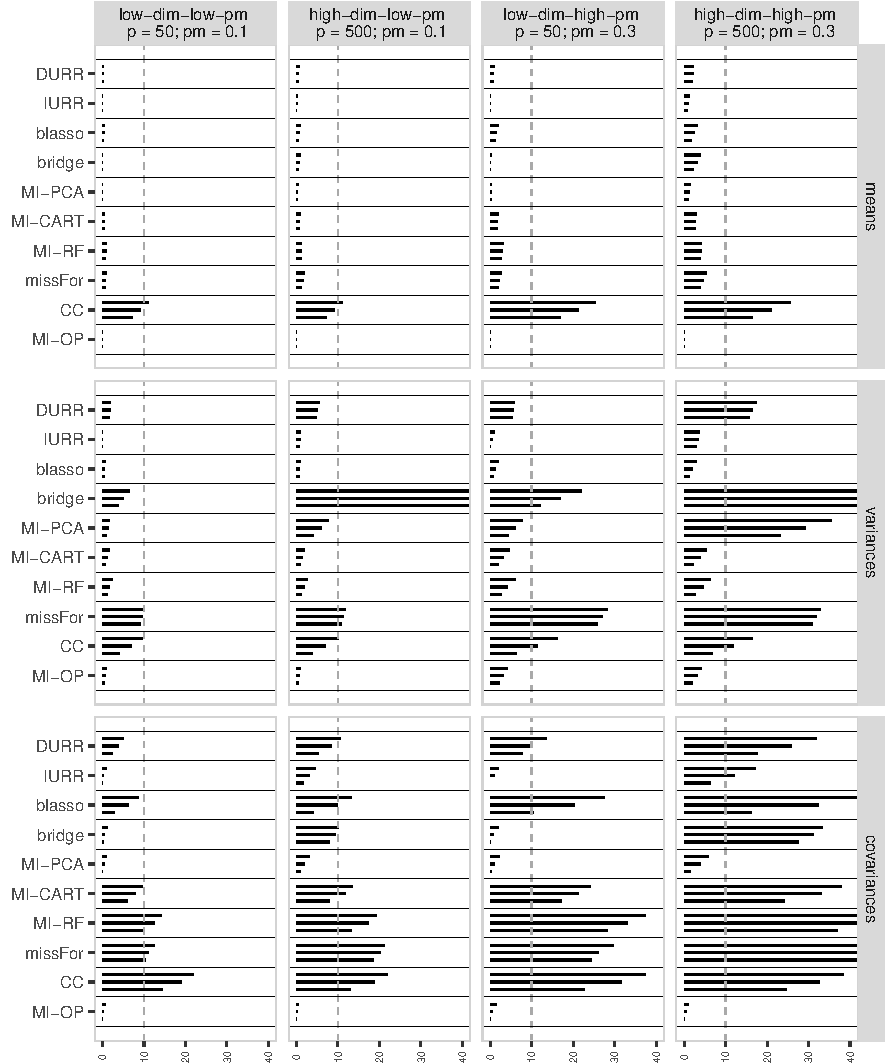
\includegraphics{../../output/graphs/exp1_bias_summy.pdf}
\caption{\label{fig:exp1bias}
	Percent Relative Bias (PRB) for item means, variances, and covariances.
	For every method, single horizontal lines, representing the PRB of a parameter estimate on 
	a single variable (or pair of variables), combine to form larger horizontal bars giving an 
	aggregate account of how each method performed across multiple variables with missing values.
	}
\end{figure}

\begin{figure}
\centering
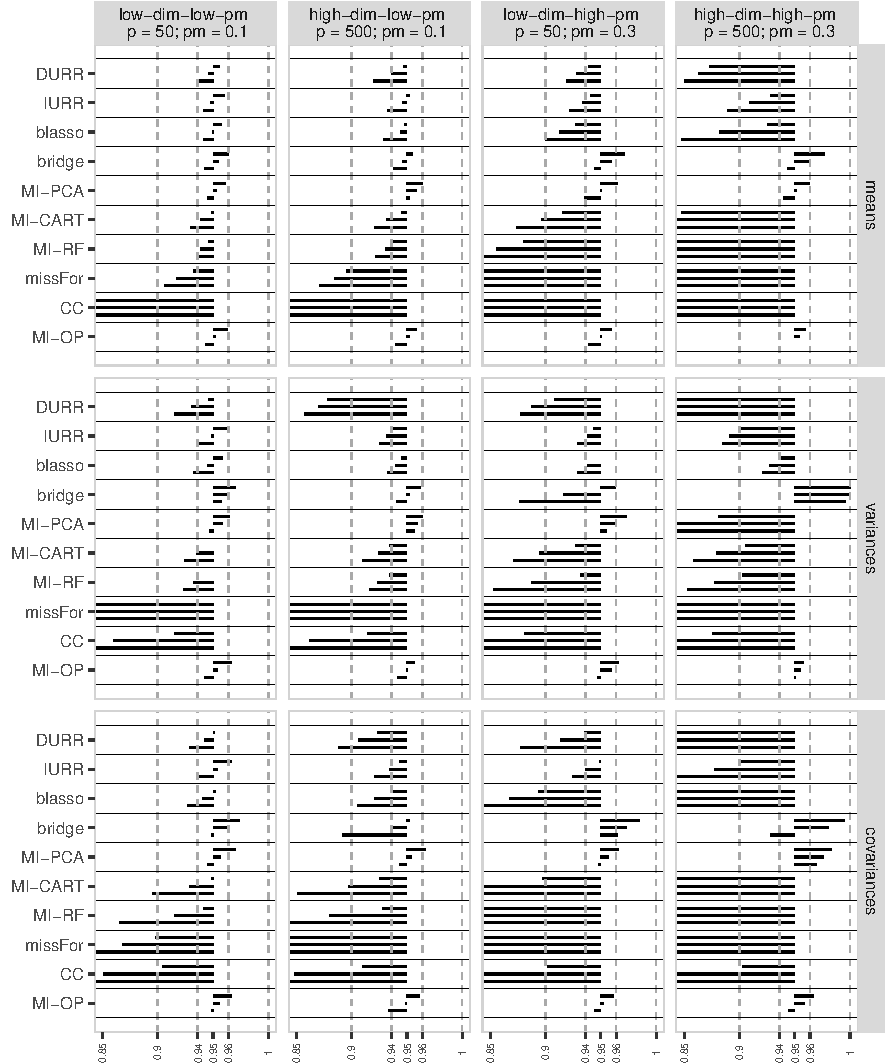
\includegraphics{../../output/graphs/exp1_CI_summy.pdf}
\caption{\label{fig:exp1cir}
	Confidence Interval Coverage (CIC) for item means, variances, and covariances. 
	For every method, single horizontal lines, representing the CIC of a parameter estimate on 
	a single variable (or pair of variables), combine to form larger horizontal bars giving an 
	aggregate account of how each method performed across multiple variables with missing values.
	}
\end{figure}
	
\FloatBarrier % stops fig:exp1cir to leave its section

